\documentclass[aspectratio=169]{beamer}

\usepackage{subcaption}

\title{Evaluación y desarrollo de \textit{eye tracking} remoto en navegadores
\textit{web}}
\author{Francisco Figari}
\date{Buenos Aires, 2022}
\titlegraphic{
\includegraphics[width=8em]{img/logo-fcen.png}}  

\setbeamertemplate{navigation symbols}{}

\setbeamertemplate{frametitle}{
  \insertsectionhead\par
  \vspace*{0.2mm}
  \insertsubsectionhead\par
  \vspace*{0.2mm}
  \insertframetitle
}

\begin{document}

% quiénes, qué, cuándo, dónde
% Juan, Gus, Bruno y yo
% estudiando
%   la aplicabilidad de eye tracking web
%   al diagnóstico de condiciones neuropsicológicas
%   a través de análisis clínicos remotos
% durante el último año
% acá
%   en el LIAA
%   en el contexto de las Pasantías de Iniciación en la Investigación en Computación

\frame{\titlepage}

\section{Motivación}

\begin{frame}{~}

  \begin{itemize}
      \item los ojos como entrada a los procesos cognitivos y estados
        emocionales de una persona
      \item frecuentemente estudiados en el contexto de la neuropsicología
        digital para estimar el comportamiento
      \item importante incluso cuando no son el foco del análisis
        (\textit{e.g.}, detección de caras)
      % utilizado también en el desarollo HMI, en el estudio de usabilidad de
      % interfaces, recientemente en el campo de la oftalmología para estimar
      % el campo visual
      \item usos en otras disciplinas
  \end{itemize}

  \begin{figure}
    \begin{subfigure}{0.49\textwidth}
      \centering
      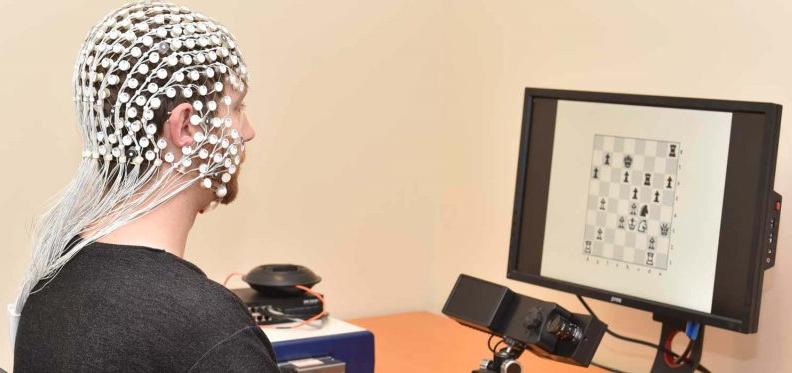
\includegraphics[width=\linewidth]{img/eye-link-eeg.jpg}
      \caption{\textit{Eye tracking} combinado con electroencefalograma}
    \end{subfigure}
    \begin{subfigure}{0.49\textwidth}
      \centering
      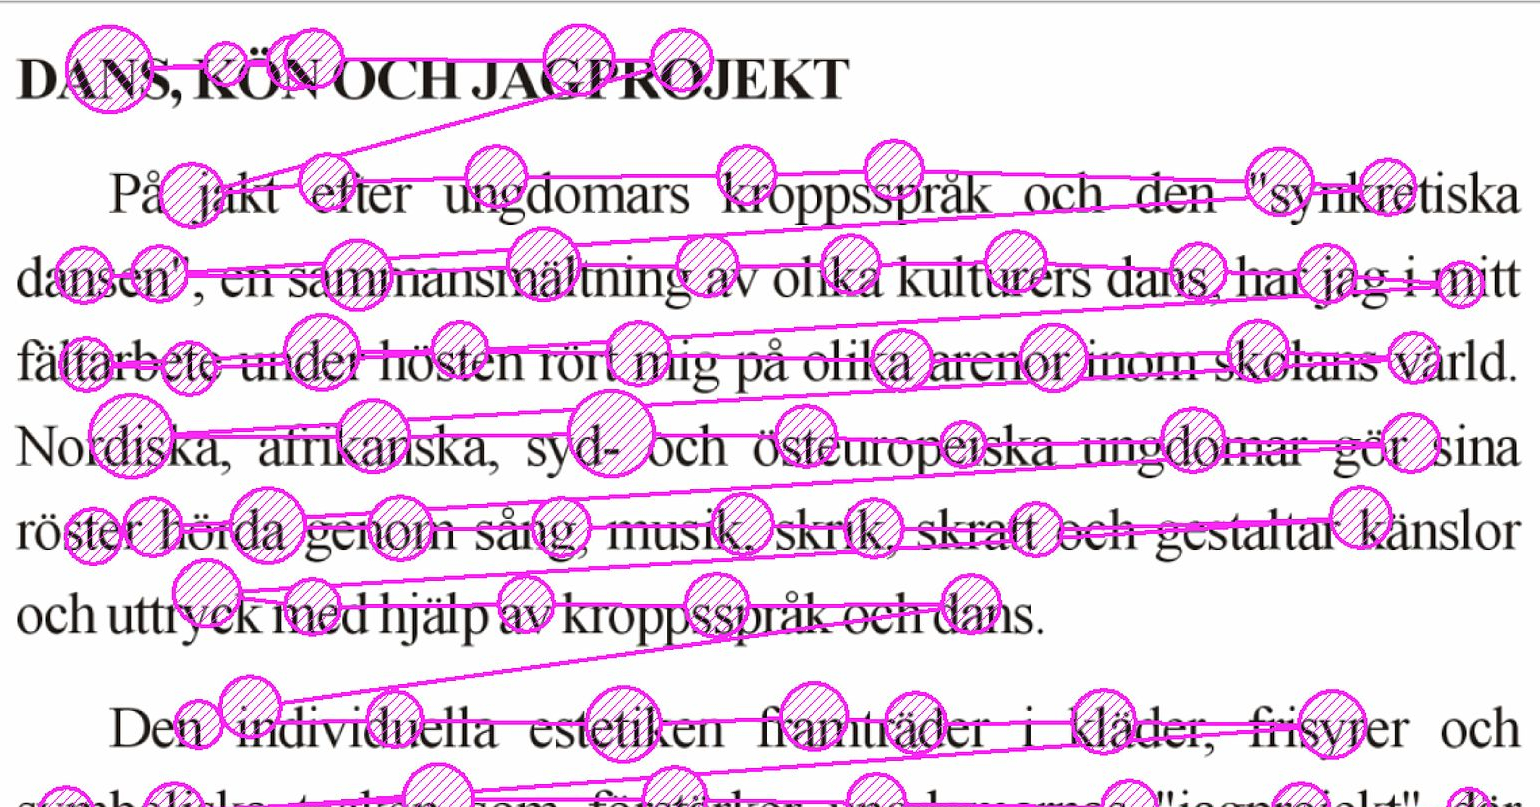
\includegraphics[width=\linewidth]{img/reading-fixations-saccades.jpg}
      \caption{Estimación de la mirada durante una tarea de lectura}
    \end{subfigure}
  \end{figure}

\end{frame}

\begin{frame}{~}

  \begin{itemize}
    \item comunmente resuelto con sistemas comerciales cerrados
    \item costos altos (entre 5000 y 40000 euros) mientras que el hardware en
      sí representa una pequeña fracción de estos (entre 200 y 600 euros)
    % si falta algún dato (e.g., la precisión del diámetro de la pupila) no
    % se lo puede saber
    \item imposibilidad de auditar la implementación
    \item necesidad de asistir a un laboratorio
  \end{itemize}

  \begin{figure}
    \begin{subfigure}{0.49\textwidth}
      \centering
      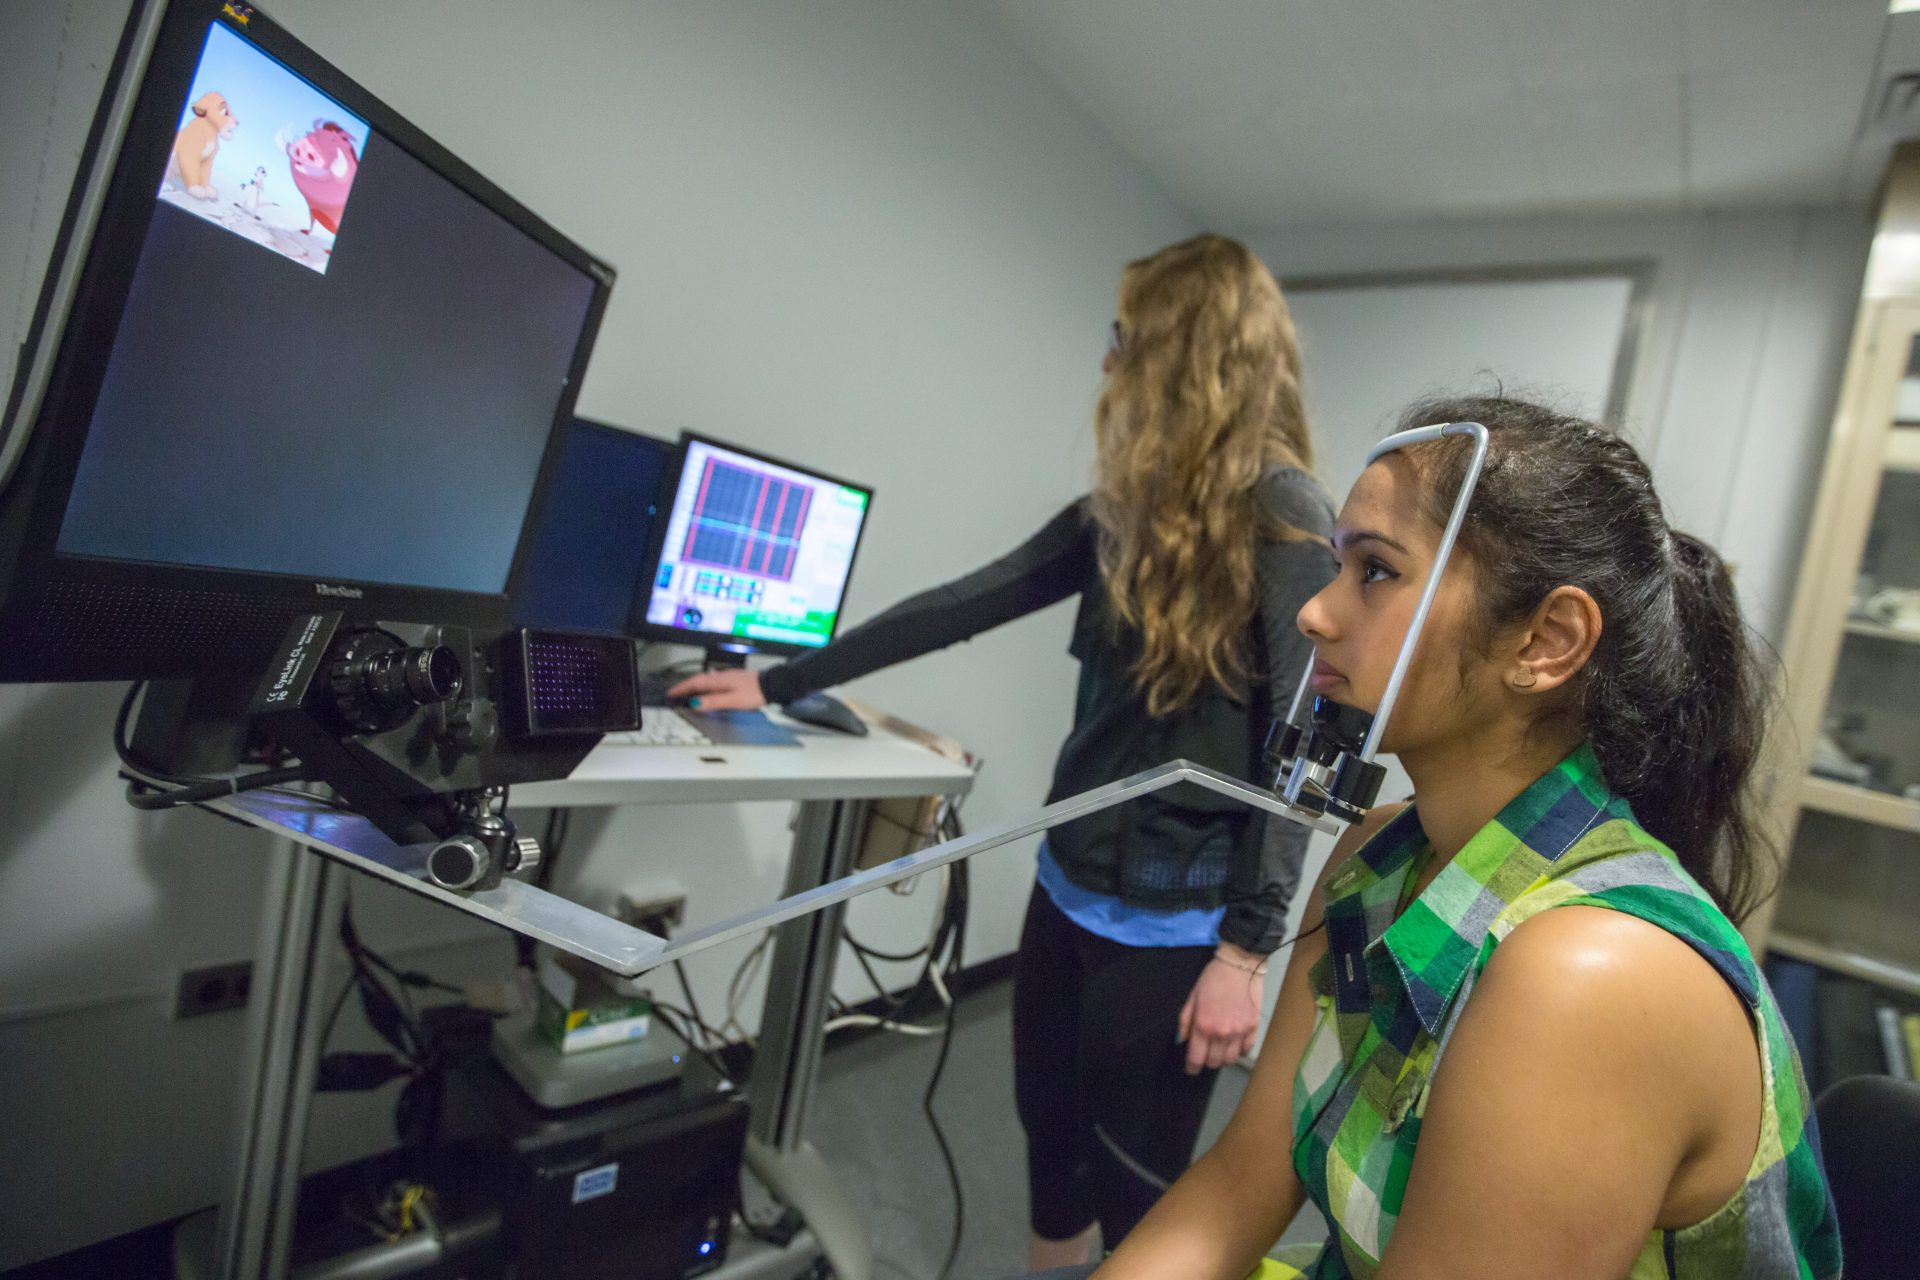
\includegraphics[width=0.6\linewidth]{img/eye-link-chinrest.jpg}
      \caption{La reestricción de movimiento facilita mantener calibrado el
      sistema}
    \end{subfigure}
    \begin{subfigure}{0.49\textwidth}
      \centering
      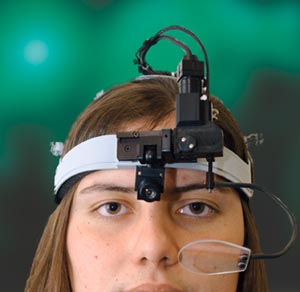
\includegraphics[width=0.5\linewidth]{img/eye-tracker-head-mounted.jpg}
      \caption{\textit{Eye tracker} montado a la cabeza}
    \end{subfigure}
  \end{figure}

\end{frame}

\begin{frame}{~}

  \begin{itemize}
    \item Interés en proveer software de \textit{eye tracking}
  \end{itemize}

  \begin{figure}
    \begin{subfigure}{0.49\textwidth}
      \centering
      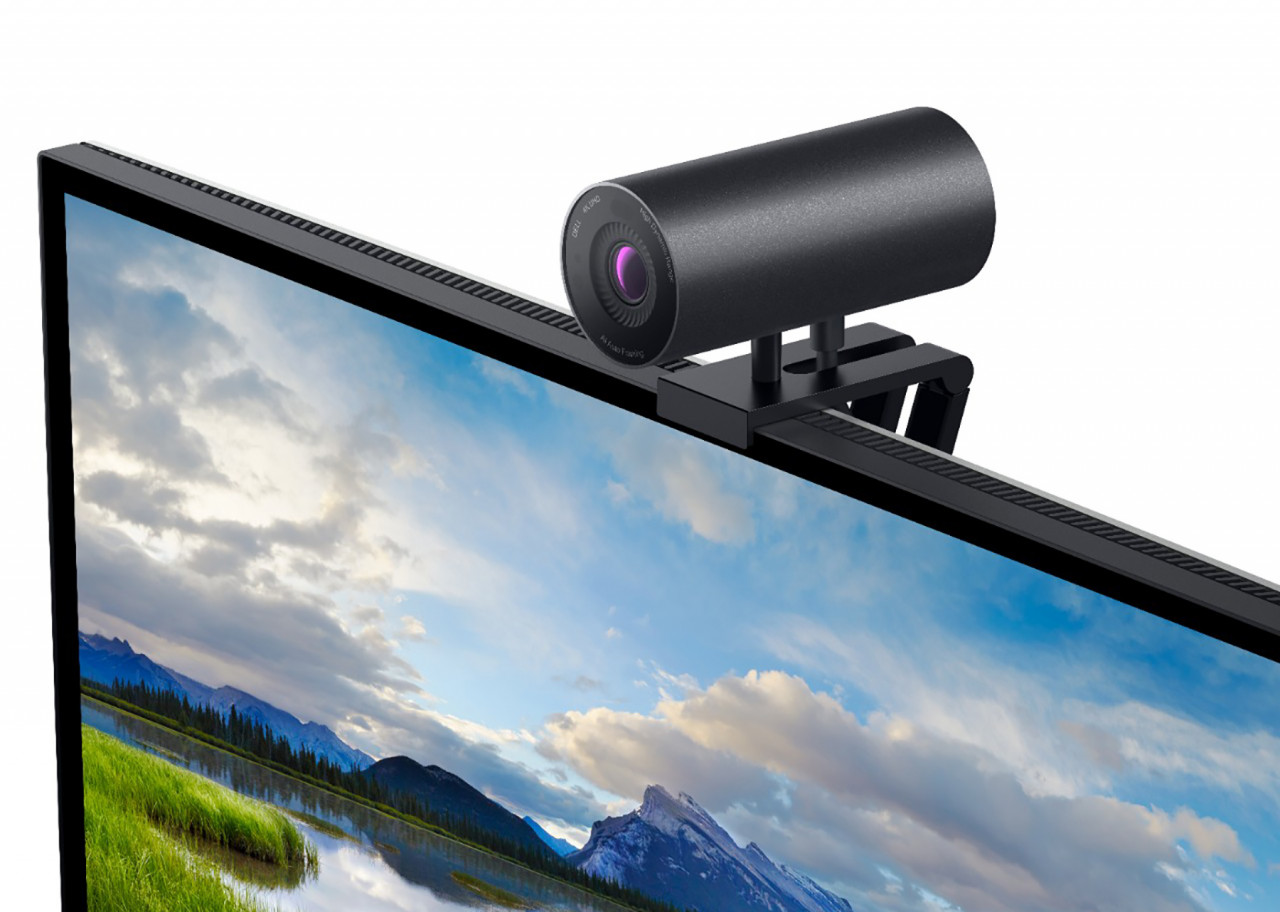
\includegraphics[width=0.6\linewidth]{img/external-webcam.jpg}
    \end{subfigure}
    \begin{subfigure}{0.49\textwidth}
      \centering
      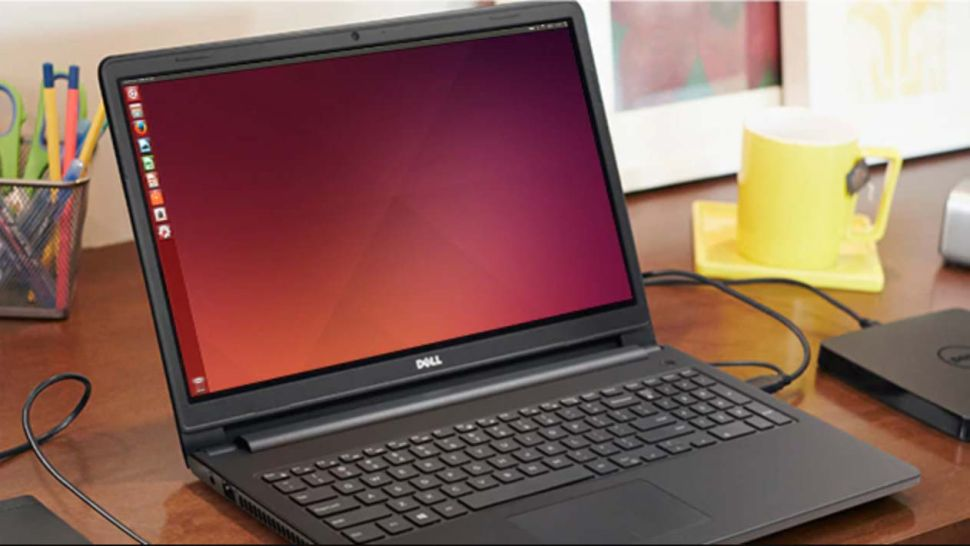
\includegraphics[width=0.6\linewidth]{img/notebook.jpg}
    \end{subfigure}
    \caption{Webcams domésticas ya disponibles}
  \end{figure}

  \begin{figure}
    \begin{subfigure}{0.49\textwidth}
      \centering
      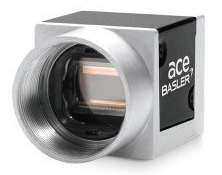
\includegraphics[width=0.35\linewidth]{img/basler-camera.jpg}
    \end{subfigure}
    \begin{subfigure}{0.49\textwidth}
      \centering
      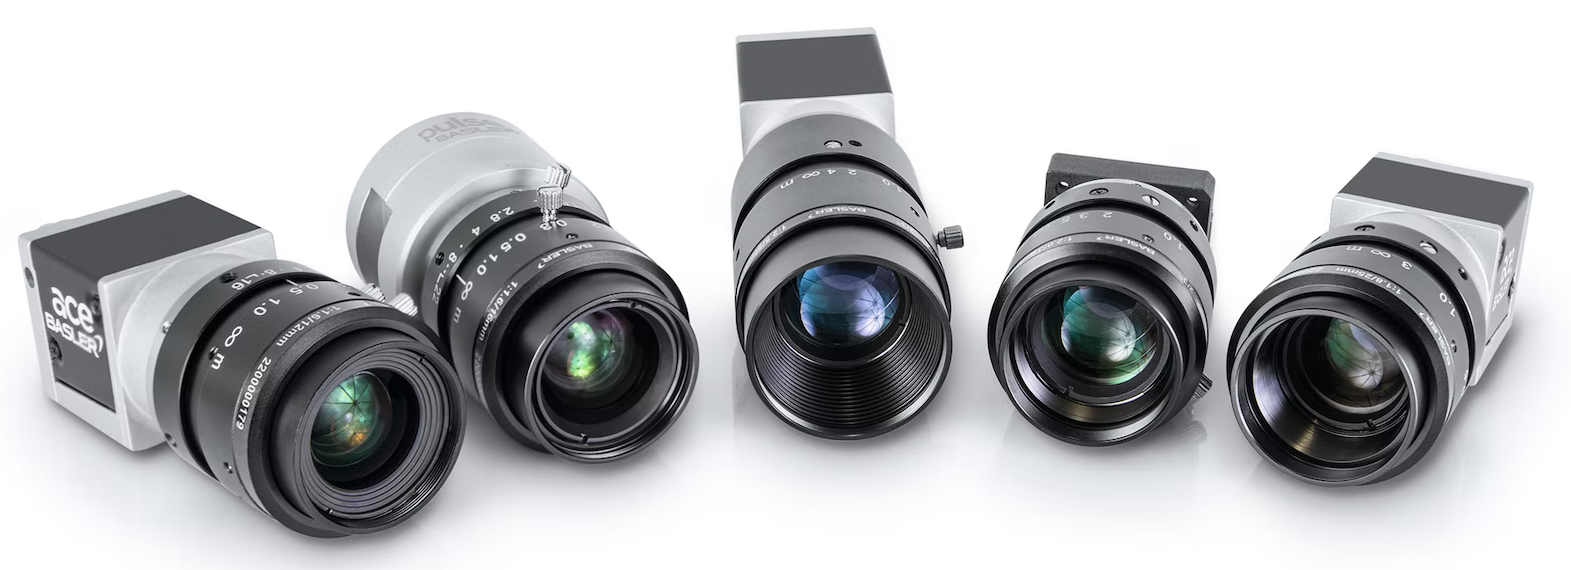
\includegraphics[width=0.6\linewidth]{img/basler-cameras-with-lens.png}
    \end{subfigure}
    \caption{Hardware profesional adquirible por una fracción del costo}
  \end{figure}

\end{frame}

\section{Objetivos}

\begin{frame}{~}

  \begin{itemize}
    \item Evaluar implementaciones recientes con similares motivaciones
    % - entender el problema
    % - definir los requerimientos
    % - establecer qué puede reutilizarse

    \item Implementar un prototipo de \textit{eye tracker} que corra en
      navegadores \textit{web} y que esté orientado a análisis clínicos
    % - adaptar lo que pudiera reutilizarse
    % - implementar los módulos que faltaran

    \item Emular análisis clínicos remotos y recolectar datos utilizando el 
      prototipo implementado

    \item Establecer la capacidad del prototipo en replicar conclusiones
      establecidas con \textit{eye trackers} profesionales de laboratorio

  \end{itemize}

\end{frame}

\section{Caso de estudio: tarea de antisacadas}

\begin{frame}{~}

. qué es?
. cómo se la diseña?
. qué procesos cogntivos permite explorar?
. qué condiciones neuropsicológicas fueron estudiadas?

\end{frame}

\section{Alternativas al \textit{eye tracking} tradicional}

\subsection{Trabajos previos}

\begin{frame}{~}

% analizamos trabajos que compartieran los objetivos de proveer software
% necesario para eye tracking, ya sea tq el implementador provea el software o
% bien reutilizando cámaras web
. PupilEXT
. PACE
. TG
. Último hablar de WG y señalar como construyen sobre PACE y WG

\end{frame}

\subsection{Implicancias del contexto de navegador \textit{web}}

\begin{frame}{~}

. hardware gratis pero limitado

. ambiente no controlado (dificultades de luz, variablidad de hardware)
  comunicación a través de interfaces web

\end{frame}

\subsection{Modelado de la mirada}

\begin{frame}{~}
. bibliografía reducida

. calibración, cómo la hago
  no hay un estándar
  necesidad de minimizar tiempo total del exp
  en cada sesión hay que recalibrar

. ausencia de invarianza frente a movimientos de cabeza
  cómo decidir cuándo se descalibró la herramienta
  importancia resaltada por ausencia de reestricciones de movimiento
\end{frame}

\section{Implementación}

\subsection{WebGazer como punto de partida}

\begin{frame}{~}
+ tiene hecho el laburo de conectar con la API de JS para extraer los frames de
  la webcam
  + localización de los ojos (TODO: Explicar facemesh acá)
+ estimación de la mirada
- calibración inadecuada
- ausencia de notificación de descalibraciones
\end{frame}

\subsection{Calibración y validación}

\begin{frame}{~}
. por qué no sirve el sistema de WG (basado en interacciones)
. cómo quedó implementado
. mejora hecha sobre WG para evitar recalcular coeficientes en cada frame
\end{frame}

\subsection{Notificación de descalibración}

\begin{frame}{~}
. cómo está implementada
. exposición de las features de WG

TODO: Pseudocódigo
\end{frame}

\subsection{Playgrounds}

\begin{frame}{~}
. interfaces lógicas
. mayor comodidad para desarrollar el sistema
\end{frame}

\section{Experimentación}

\begin{frame}{~}
. cómo se diseño cada instancia
. cómo se distribuyeron
. mencionar mejora a WG sobre el paquete de facemesh
\end{frame}

% me voy a concentrar directo en lo que quedó armado para la segunda instancia
\section{Código de análisis}

\subsection{Características de los datos}

\begin{frame}{Frecuencias de muestreo}

TODO: Plots

\end{frame}

\begin{frame}{Anchos de pantalla}

TODO: Plots

\end{frame}

\begin{frame}{Estimaciones desviadas}

TODO: Plots

\end{frame}

\subsection{Limpieza y normalización}

% No hacer mucho hincapié acá y comentar que en cualquier caso está disponible
% la implementación
\begin{frame}{~}

TODO: Ejemplos de datos descartados
TODO: Ejemplos de cómo quedan los datos luegos de la normalización

\end{frame}

\subsection{Detección de sacadas}

\begin{frame}{~}
TODO: Pseudocódigo
\end{frame}

\section{Resultados}

\begin{frame}{Experimentación insuficiente}
TODO: tablas datos filtrados
TODO: plots edades
\end{frame}

\begin{frame}{Resultados generales replicados}
TODO: tablas
\end{frame}

\begin{frame}{Grupos incorrectos con baja representatividad}
TODO: tablas con datos
. posiblemente relacinado al mecanismo de detección de sacadas implementado
TODO: Plots de sacadas no detectadas
\end{frame}

\section{Conclusiones}

\begin{frame}{~}
. qué se obtuvo
. potencial para realizar análisis clínicos pero muy verde y muy por debajo de
  la precisión alcanzable con et profesionales
. protocolo de utilización
\end{frame}

\subsection{Limitaciones}

\begin{frame}{Implementativas}
. bajas frecuencias
. pestañeos
. estimación del tamaño de la pantalla
. imprecisión en la duración de cada frame, problemático si se quiere mostrar
  un estímulo durante una corta duración de tiempo
\end{frame}

\begin{frame}{Experimentales}
. proporción de datos filtrados demasiado elevada
. necesidad de revisar la causa de las altas tasas de correctitud obtenidas
. representatividad de distintos grupos etarios
\end{frame}

\subsection{Trabajo futuro}

\begin{frame}{Análisis de datos}
. Investigar e implementar mecanismos estándares de detección de sacadas, lo
  cual podría basarse en la previa construcción de un dataset etiquetado de
  sacadas
. Revisar criterios de exclusión para asegurarse de no estar filtrando datos
  válidos
. Realizar nuevas rondas de experimentación, estimando previamente la cantidad
  de ensayos necesarios para asegurar cantidades suficientes en los grupos
  incorrectos y en los distintos grupos etarios
\end{frame}

\begin{frame}{Análisis de sensibilidad}
. propuesta sobre experimento para recolectar datos y establecer métricas de
  calidad sobre las estimaciones obtenidas por la herramienta
TODO: Acá combinar un poco lo que quedó en la tesis y lo que pensé para
      sensitivity analysis
\end{frame}

\begin{frame}{Prototipo desarrollado}
. optimizar frecuencia de muestreo
. reexplorar detección de descalibraciones y qué significa que el sistema esté
  descalibrado
. mejorar la calibración, generalizarla a más puntos de interés
. detección de pestañeos
. estimación del tamaño de la pantalla y posibilidad de mostrar estímulos en
  grados
. verificación de condiciones iniciales
TODO: Extender con lo que haya escrito en la tesis
\end{frame}

\begin{frame}{\textit{Eye tracking} en navegadores \textit{web}}
. extender bibliografía que aplique a nuestro contexto
. eye tracking web no podría atacar algunos problemas que sí puede el eye
  tracking tradicional, pero al ser remoto y de bajo costo es posible que
  permita atacar nuevos problemas. Deben entonces buscarse tales problemas
\end{frame}

\end{document}
